\documentclass[a4paper,11pt]{article}
\usepackage[italian]{babel}
\usepackage[utf8]{inputenc}
\usepackage{csquotes}
\usepackage[margin = 1.4in]{geometry}
\usepackage{amsmath}
\usepackage{centernot}
\usepackage{amsfonts}
\usepackage{tcolorbox}
\usepackage{float}
\usepackage[font=scriptsize]{caption}
\usepackage[framemethod=tikz]{mdframed}
\usepackage[
backend=biber,
style=alphabetic,
]{biblatex}
\addbibresource{citations.bib}
\newmdenv[innerlinewidth=0.5pt,roundcorner=4pt,linecolor=lightgray,innerleftmargin=6pt,
innerrightmargin=6pt,innertopmargin=6pt,innerbottommargin=6pt]{myblock}
\begin{document}
\title{\textbf{Transistor BJT}

1° turno tavolo 5}
\author{Stefano Doria 0001093903 \and Giuseppe Luciano 0001077643}

\date{Novembre 2024}

\maketitle

\section{Abstract}

Items that are cited: \textit{The \LaTeX\ Companion} book \cite{latexcompanion} together with Einstein's journal paper \cite{einstein} and Dirac's book \cite{dirac}---which are physics-related items. Next, citing two of Knuth's books: \textit{Fundamental Algorithms} \cite{knuth-fa} and \textit{The Art of Computer Programming} \cite{knuth-acp}.

\section{Introduzione}
in questo esperimento si è osservata la corrente in uscita dal collettore di un transistor a giunzione bipolare (BJT) nella configurazione a base comune in regione attiva e si sono misurati diverse grandezze tipiche del transistor in queste condizioni.

Un transistor BJT pnp è un dispositivo formato da tre porzioni di semiconduttore: un emettitore e un collettore drogate $p$, e una base, molto meno drogata con un drogaggio di tipo $n$. Si ottiene così la geometria mostra in figura \ref{fig::pnp}, in cui è possibile individuare due giunzioni p-n. Tale dispositivo viene poi inserito in un circuito, collegando i terminali relativi a base, emettitore e collettore in modo che uno di questi risulti comune agli altri due, che a questo punto verranno considerati uno come input e l'altro come output. Avendo collegato a tensione diversa le tre porzioni del transistor si sono polarizzate le due giunzioni al suo interno.

\begin{figure}[ht]
\centering
    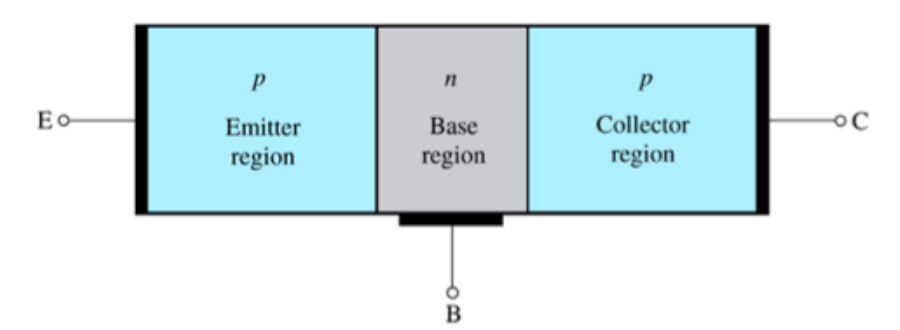
\includegraphics[width=0.7\linewidth]{pictures/pnp.png}
    \caption{Schematizzazione transistor BJT pnp. Si distinguono le tre regioni drogate $p$ e $n$}
    \label{fig::pnp} 
\end{figure}

Nel caso che si sta presentando è stato scelto l'emettitore come terminale comune, configurazione in cui la base rappresenta l'input mentre il collettore l'output. Sono dunque state applicate differenze di potenziale $V_{BE} < 0$ (d.d.p. tra base ed emettitore) e $V_{BC} > 0$ (d.d.p. tra base e collettore) in modo che la giunzione base-emettitore risultasse polarizzata direttamente mentre quella base-collettore inversamente, mettendosi in quella che è detta regione attiva del transistor.

In queste condizioni, che producono amplificazioni sia in corrente sia in tensione, la corrente in uscita in funzione di quella in ingresso è data dalla relazione \ref{eq::correnti}

\begin{equation}
I_C = \beta_F I_B
\label{eq::correnti}
\end{equation}

dove $I_C$ è la corrente in uscita del collettore, $I_B$ è la corrente in entrata della base e $\beta_F$ è il coefficiente di guadagno in configurazione ad emettitore comune. Questo parametro è poi stato valutato come mostrato nella relazione \ref{eq::beta}

\begin{equation}
    \label{eq::beta}
\beta_F = \Delta I_C / \Delta I_B
\end{equation}

per correnti valutate a stessi valori di tensione.

Contrariamente a quanto ci si attenderebbe dall'equazione \ref{eq::correnti}, la caratteristica I-V in uscita, per valori di tensione oltre qualche decimo di volt, non mostra un andamento di corrente costante, bensì assume la forma riportata nella relazione \ref{eq::caratt_uscita} %qui direi anche che ciò è causa delle approssimazioni apportate alle leggi di Emers Moll o come si scrivono

\begin{equation}
    \label{eq::caratt_uscita}
    V_{CE} = V_A + R_O I_C \hspace{10mm} \longleftrightarrow  \hspace{10mm} I_C = V_{CE}/R_O - V_A/R_O
\end{equation}

dove $V_{CE}$ è la d.d.p. tra collettore ed emettitore, $V_A$ è la tensione di Early e $R_O$ è la resistenza in uscita per un valore fissato di $I_B$. Tale andamento non costante in corrente è conseguenza della diminuzione della larghezza effettiva della base nella quale la depletion region della giunzione collettore-base polarizzata inversamente penetra sempre più profondamente all'aumentare in modulo di $V_{BC}$, e dunque di $V_{CE}$. Ciò prende il nome di effetto Early ed è quantificato da $V_A$, che rappresenta l'intercetta di queste rette con l'asse delle tensioni.

Per valori di $V_{CE}$ molto piccoli in modulo si ha che la giunzione collettore-base non risulta polarizzata inversamente ma direttamente, ponendo così in transistor in un'altra regione di funzionamento chiamata regione di saturazione.

Un ultimo parametro di interesse che si cita è la conduttanza in uscita a $I_B$ fissata, che è il reciproco di $R_O$ e che indichiamo come $G_O$.

%vedere di scrivere questa introduzione in maniera più sintetica

\section{Metodo sperimentale}

Durante l'esperimento si sono usati un multimetro FLUKE 77 IV per le misure di corrente ed un oscilloscopio GOS-622B (modello 1) per le misure di tensione. Altri dispositivi utilizzati sono un generatore di tensione continua che forniva una d.d.p. di -5 V, un potenziometro da 100 k$\Omega$ uno da 1 k$\Omega$ per modulare tensione e corrente rispettivamente in entrata e in uscita dal transistor. In figura \ref{fig::apparato} si riporta l'apparato sperimentale mentre in figura \ref{fig::circuito} viene mostrato uno schema del circuito utilizzato durante l'esperimento.

\begin{figure}
    \centering
    \begin{minipage}{0.5\textwidth}
        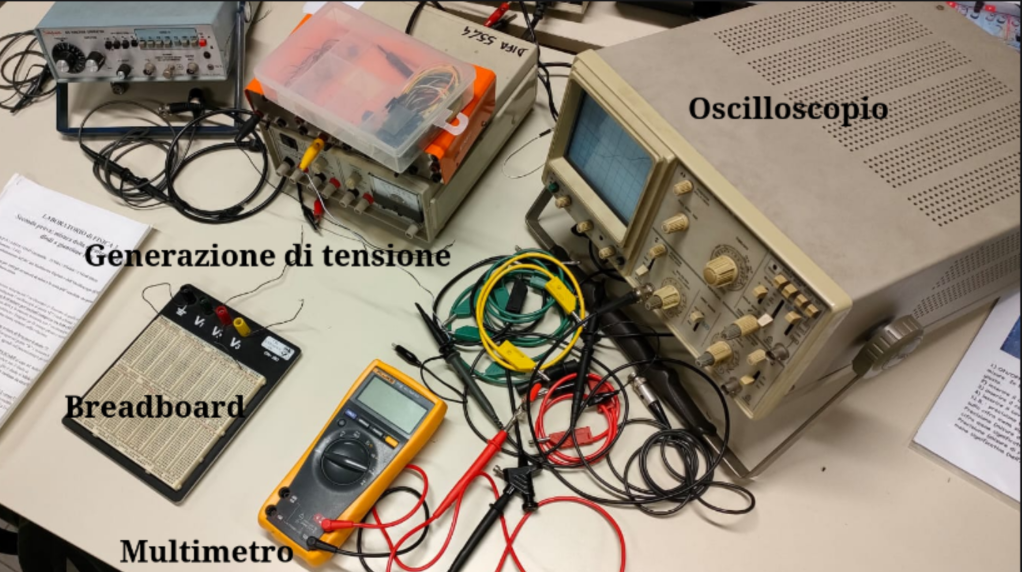
\includegraphics[width=1\linewidth]{pictures/apparato.png}
          \caption{\textit{\textcolor{gray}{L'immagine mostra l'apparato sperimentale impiegato, con l'oscilloscopio, il multimetro, la breadboard e il generatore di tensione. }}}
        \label{fig::apparato}
    \end{minipage}
    \hfill
    \begin{minipage}{0.49\textwidth}
        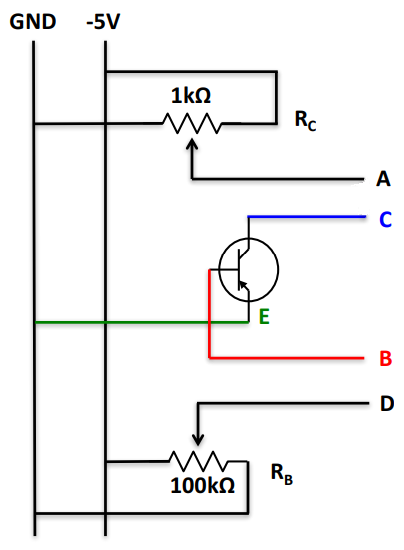
\includegraphics[width=0.6\linewidth]{pictures/circuito.png}
        \centering
        \caption{\textit{\textcolor{gray}{Schema del circuito usato nell'esperimento. Il simbolo cerchiato rappresenta il transistor pnp, mentre $R_B$ e $R_C$ sono i potenziometri usati per modulare tensione e corrente rispettivamente su base (B) e collettore (C). L'emettitore (E) collegato al ground è il terminale comune.}}}
        \label{fig::circuito}
    \end{minipage}
\end{figure}

Si sono dunque effettuate due serie di misure della caratteristica I-V in uscita fissando la $I_B$ in entrata prima a -200 $\mu$A e poi a -100 $\mu$A. 

Per fissare i valori di $I_B$ si sono circuitati i punti A e C del circuito e si è collegato il multimetro tra i punti B e D, così che misurasse $I_B$. Si è dunque utilizzato il potenziometro da 100 k$\Omega$ per selezionare il valore di corrente desiderato.

Per la misura della caratteristica I-V in uscita si sono invece circuitati i punti B e D, si è collegato il multimetro tra i punti A e C e si è inserito l'oscilloscopio nel punto C, così che i due strumenti potessero misurare rispettivamente corrente e tensione in uscita dal collettore. Per prendere misure a diversi valori di tensione, questa veniva variata attraverso il potenziometro da 1 k$\Omega$,

Un problema durante l'acquisizione dati per la caratteristica in uscita è che i transistor tendono a scaldarsi molto rapidamente quando vi scorre corrente quindi il semiconduttore di cui il dispositivo è fatto varia le sue caratteristiche nel tempo, il che portava a valori di corrente misurati per una data tensione non stabili, ma che aumentavano col tempo. Questo a causa del fatto che all'aumentare della temperatura più portatori monoritari potevano venir creati aumentando di conseguenza la corrente. Per mitigare quest'effetto si sono adottate una serie di prassi. Innanzitutto si sono effettuate prima le misure con $I_B$ in modulo maggiore, e per ciascuna delle prese dati a $I_B$ costante si è cominciato ad acquisire per i valori di tensione più alti andando poi a scendere. Inoltre si è tenuto spento il generatore di tensione quando non fosse necessario per impostare la tensione successiva e si sono registrati i valori di corrente ad una certa tensione sia appena acceso il generatore sia dopo 10s.
%magari specifichiamo come nella precedente relazione che si è selezionata di volta in volta la sensibilità sull'oscilloscopio più alta e si è fatto in modo che i punti non si trovassero ai margini superiori ed inferiore del display dell'oscilloscopio per non deformare il segnale (copia pure quello che avevamo detto in precedenza) poi bisogna anche mettere nel testo delle citazioni a diversi articoli magari nella parte delle equazioni. specificherei anche che dopo aver finito la prima curva abbiamo atteso una decina di minuti prima di iniziare la caratteristica successiva per riportare a temperatura aumbiente il transistor, non è una cosa così trascurabile. infine non sarebbe male anche aggiungere qualche valore di riferimento per le tensioni in prossimità del ginocchio ecc     

Infine si riferisce che le misure sono state effettuate agli stessi valori di tensione uscita per le due diverse $I_B$ fissate, in modo da poter comodamente calcolare $\beta_F$ con l'equazione \ref{eq::beta}. Inoltre, visto che l'interesse era per la caratteristica I-V per la regione attiva del transistor, si sono presi soprattutto punti in quella regioni per tensioni non troppo piccole, aumentandone però il numero in prossimità della regione di saturazione per poter individuare al meglio dove avvenisse la transizione. 

\section{Risultati}

\subsection{Dati}
Nelle tabelle \ref{tab::dati_100} e \ref{tab::dati_200} si riportano le misure di tensione corrente con corrente sulla base impostata rispettivamente a (100 $\pm$ 22) $\mu \mathrm{A}$ e (200 $\pm$ 23) $\mu \mathrm{A}$. Invece nella tabella \ref{tab::risultati} si riportato i valori della tensione di Early, la resistenza in uscita, indicata con b, la conduttanza, indicata con g ed il fattore di guadagno indicato con $\beta$.

\begin{minipage}{0.4\textwidth}
        \[
\begin{array}{|c|c|}
\hline
\text{Tensione (V)} & \text{Corrente (mA)}
\\ \hline
4.00 \pm 0.16 f.s. 1 & 17.75 \pm 0.17 \\ 
3.60 \pm 0.15 f.s. 1 & 17.73 \pm 0.17 \\ 
3.20 \pm 0.14 f.s. 1 & 17.53 \pm 0.16 \\ 
2.80 \pm 0.10 f.s. 0.5 & 17.30 \pm 0.16 \\ 
2.600 \pm 0.093 f.s. 0.5 & 17.13 \pm 0.16 \\ 
2.400 \pm 0.088 f.s. 0.5 & 16.97 \pm 0.16 \\ 
2.200 \pm 0.083 f.s. 0.5 & 16.80 \pm 0.16 \\ 
2.000 \pm 0.078 f.s. 0.5 & 16.67 \pm 0.16 \\ 
1.800 \pm 0.074 f.s. 0.5 & 16.52 \pm 0.15 \\ 
1.600 \pm 0.069 f.s. 0.5 & 16.37 \pm 0.15 \\ 
1.400 \pm 0.065 f.s. 0.5 & 16.19 \pm 0.15 \\ 
1.200 \pm 0.041 f.s. 0.2 & 16.03 \pm 0.15 \\ 
1.100 \pm 0.039 f.s. 0.2 & 15.95 \pm 0.15 \\ 
1.000 \pm 0.036 f.s. 0.2 & 15.83 \pm 0.15 \\ 
0.900 \pm 0.034 f.s. 0.2 & 15.73 \pm 0.15 \\ 
0.800 \pm 0.031 f.s. 0.2 & 15.62 \pm 0.15 \\ 
0.700 \pm 0.029 f.s. 0.2 & 15.48 \pm 0.15 \\ 
0.600 \pm 0.027 f.s. 0.2 & 15.35 \pm 0.14 \\ 
0.500 \pm 0.018 f.s. 0.1 & 15.17 \pm 0.14 \\ 
0.400 \pm 0.016 f.s. 0.1 & 14.89 \pm 0.14 \\ 
0.300 \pm 0.010 f.s. 0.05 & 14.15 \pm 0.13 \\ 
0.2000 \pm 0.0078 f.s. 0.05 & 11.56 \pm 0.11 \\ 
0.1000 \pm 0.0036 f.s. 0.02 & 3.28 \pm 0.040 \\
\hline
\end{array} \label{tab::dati_100}
\]
    \end{minipage}
    \hfill %lui mette lo spazio in mezzo
    \begin{minipage}{0.4\textwidth}
        \[
\begin{array}{|c|c|}
\hline
\text{Tensione (V)} & \text{Corrente (mA)} \\ \hline
4.00 \pm 0.16 f.s. 1 & 35.61 \pm 0.32 \\ 
3.60 \pm 0.15 f.s. 1 & 35.19 \pm 0.32 \\ 
3.20 \pm 0.14 f.s. 1 & 34.63 \pm 0.31 \\ 
2.80 \pm 0.10 f.s. 0.5 & 33.76 \pm 0.31 \\ 
2.60 \pm 0.09 f.s. 0.5 & 33.43 \pm 0.30 \\ 
2.40 \pm 0.09 f.s. 0.5 & 33.07 \pm 0.30 \\ 
2.20 \pm 0.08 f.s. 0.5 & 32.46 \pm 0.29 \\ 
2.00 \pm 0.08 f.s. 0.5 & 32.12 \pm 0.29 \\ 
1.80 \pm 0.07 f.s. 0.5 & 31.94 \pm 0.29 \\ 
1.60 \pm 0.07 f.s. 0.5 & 31.39 \pm 0.28 \\ 
1.40 \pm 0.07 f.s. 0.5 & 31.16 \pm 0.28 \\ 
1.20 \pm 0.04 f.s. 0.2 & 30.73 \pm 0.28 \\ 
1.10 \pm 0.04 f.s. 0.2 & 30.44 \pm 0.28 \\ 
1.00 \pm 0.04 f.s. 0.2 & 30.05 \pm 0.27 \\ 
0.90 \pm 0.03 f.s. 0.2 & 29.79 \pm 0.27 \\ 
0.80 \pm 0.03 f.s. 0.2 & 29.38 \pm 0.27 \\ 
0.70 \pm 0.03 f.s. 0.2 & 28.93 \pm 0.26 \\ 
0.60 \pm 0.03 f.s. 0.2 & 28.16 \pm 0.26 \\ 
0.50 \pm 0.02 f.s. 0.1 & 27.14 \pm 0.25 \\ 
0.40 \pm 0.02 f.s. 0.1 & 25.44 \pm 0.23 \\ 
0.30 \pm 0.01 f.s. 0.05 & 22.92 \pm 0.21 \\ 
0.20 \pm 0.01 f.s. 0.05 & 18.11 \pm 0.17 \\ 
0.100 \pm 0.004 f.s. 0.02 & 5.83 \pm 0.062 \\ \hline

\end{array}\label{tab::dati_200}
\]    
    \end{minipage}


L'oscilloscopio aveva diverse possibili scelte per il valore di ogni divisione presente sul display (5 V, 2 V, 1 V, 0.5 V, 0.2 V, 0.1 V, 50 mV, 20 mV, 10 mV, 5 mV). Nel calcolo dell'incertezza l'errore stimato sulla lettura è stato preso come un decimo del fondo scala, in quanto il segnale si presentava in modo molto stabile e con rumore minimo. Il riferimento a zero per la tensione sullo strumento è stato fissato usando un fondo scala di 5 mV, quindi l'errore associatovi è 0.5 mV. Per calcolare l'incertezza associata a ogni misura si sono sommati in quadratura l'errore sullo zero, l'errore sulla lettura e l'errore del costruttore, pari al 3 \% del valore misurato. L'incertezza così ottenuta è stata considerata casuale.
 
Il multimetro aveva una risoluzione di 1 $\mathrm{mV}$ sulle misure di potenziale in corrente continua su fondo scala di 6 $\mathrm{V}$ con accuratezza dello 0.3 $\%$ sulla lettura più un digit. Per le misure con l'amperometro in corrente continua vi è una risoluzione di 0.01 $\mathrm{mA}$ su fondo scala di 60 $\mathrm{mA}$ ed accuratezza del 1.5 $\%$ sulla lettura più due digit. Le incertezze ottenute per le misure con il multimetro si sono considerate massime.

\subsection{Analisi Dati} 

Nella figura \ref{graph::curve} si riportano la curve caratteristiche in uscita del transistor BJT. Si nota complessivamente un buon riscontro visivo soprattutto per quanto riguarda la curva con una corrente di base di $I_{100}$. Invece per quanto riguarda la curva con $I_{200}$ si possono osservare delle leggere fluttuazioni rispetto al valore corrispondente nella linea di fit.

Nella tabella \ref{tab::risultati} si riportano i risultati dell'analisi mediante fit per i valori della tensione di Early, la resistenza in uscita ed il guadagno di corrente per entrambe le caratteristiche

\begin{figure}[ht]
\centering
    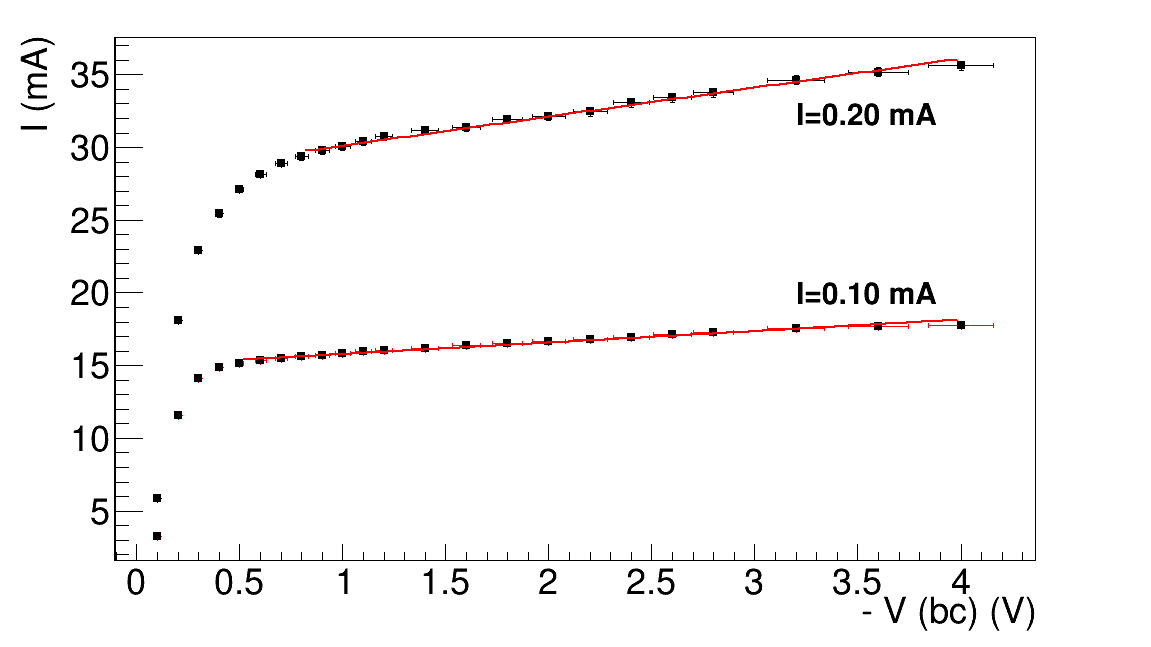
\includegraphics[width=0.7\linewidth]{pictures/g_tot_mean.png}
    \caption{\textit{\textcolor{gray}{La foto mostra le due curve di calibrazione a confronto, si sottolinea come da convenzione l'asse delle ascisse è riportato col segno invertito}}}
    \label{graph::curve} 
\end{figure}


\begin{table}[htbp] % Aggiunto ambiente table per la numerazione e il posizionamento
\begin{center}
\begin{tabular}{ |c|c|c| }
\hline
risultati & I = 100 $\mu$A & I = 200 $\mu$A \\ 
\hline
$V_{Early}$ & 19.0 $\pm$ 1.1 mV & 14.11 $\pm$ 0.76 V \\  
\hline
b & 1.264 $\pm$ 0.065 k$\Omega$ & 0.502 $\pm$ 0.024 k$\Omega$ \\
\hline
g & 0.791 $\pm$ 0.041 mS & 1.994 $\pm$ 0.096 mS \\
\hline
$\beta$ & \multicolumn{2}{|c|}{160 $\pm$ 140} \\
\hline
\end{tabular}
\caption{\textit{\textcolor{gray}{La tabella mostra i risultati ottenuti dai fit. In ordine dall'alto vengono riportati la tensione di Early, la resistenza in uscita, la conduttanza e il fattore di guadagno.}}}
\label{tab::risultati}
\end{center}
\end{table}



\section{Conclusioni}
Per la caratteristica con tensione di base di $I_{100}$ si sono ottenuti dai fit ... Come atteso il valore..
con un $\tilde\chi^2$ di 0.61

Per la caratteristica con tensione di base di $I_{200}$ si sono ottenuti dai fit ... Come atteso il valore..
con un $\tilde\chi^2$ di 0.39.

Si nota inoltre come l'aumento di temperatura durante la fase di misurazione abbia impattato maggiormente quando la corrente sulla base aveva il suo valore maggiore, questo poiché si notano visivamente delle fluttuazioni più evidenti rispetto ai valori previsti dal fit sopratutto nei punti compresi nel range di 1 V e 3 V dove le correnti risultavano importanti ed il transistor ha avuto modo di riscaldarsi a causa dei punti presi precedentemente.
Si osservano  valori di $\tilde\chi^2$ di poco inferiori all'unità, un ottimo accordo fra i dati ed il modello supportato da un eccellente riscontro visivo. Nonostante questo però essendo valori è possibile che una sovrastima delle incertezze. Quest'ultima ipotesi è supportata dal fatto che per i valori di corrente di base maggiori si osserva un peggior riscontro visivo ma un migliore $\tilde\chi^2$ a causa delle incertezze maggiori sulle misure di corrente.
%prima che mi scanni... so che è sbagliatissima come cosa ma mi era venuta in mente un po' come appunto per il futuro detto questo sono in ritardissimo, speriamo per il treno


%se vuoi 
Si nota inoltre che la corrente $(0.02 \pm 0.02)$ $ \mathrm{mA}$ misurata con il multimetro a generatore di tensione spento risulta essere compatibile con zero.



\medskip

\printbibliography


% I_100 no media

%I_200 no media
\[
\begin{array}{|c|c|}
\hline
\text{Valore (Tensione (V))} & \text{Valore (Corrente mA)} \\ \hline
4.00 \pm 0.16 & 35.38 \pm 0.32 \\ 
3.60 \pm 0.15 & 34.99 \pm 0.31 \\ 
3.20 \pm 0.14 & 34.47 \pm 0.31 \\ 
2.80 \pm 0.10 & 33.60 \pm 0.30 \\ 
2.60 \pm 0.09 & 33.28 \pm 0.30 \\ 
2.40 \pm 0.09 & 32.94 \pm 0.30 \\ 
2.20 \pm 0.08 & 32.28 \pm 0.29 \\ 
2.00 \pm 0.08 & 31.99 \pm 0.29 \\ 
1.80 \pm 0.07 & 31.86 \pm 0.29 \\ 
1.60 \pm 0.07 & 31.29 \pm 0.28 \\ 
1.40 \pm 0.07 & 31.07 \pm 0.28 \\ 
1.20 \pm 0.04 & 30.69 \pm 0.28 \\ 
1.10 \pm 0.04 & 30.40 \pm 0.27 \\ 
1.00 \pm 0.04 & 30.01 \pm 0.27 \\ 
0.90 \pm 0.03 & 29.76 \pm 0.27 \\ 
0.80 \pm 0.03 & 29.36 \pm 0.27 \\ 
0.70 \pm 0.03 & 28.92 \pm 0.26 \\ 
0.60 \pm 0.03 & 28.16 \pm 0.26 \\ 
0.50 \pm 0.02 & 27.14 \pm 0.25 \\ 
0.40 \pm 0.02 & 25.44 \pm 0.23 \\ 
0.30 \pm 0.01 & 22.92 \pm 0.21 \\ 
0.20 \pm 0.01 & 18.11 \pm 0.17 \\ 
0.10 \pm 0.00 & 5.83 \pm 0.06 \\ \hline
\end{array}
\]

%I_100 media
\[
\begin{array}{|c|c|}
\hline
\text{Valore (Tensione (V))} & \text{Valore (Corrente mA)} \\ \hline
4.00 \pm 0.16 & 17.75 \pm 0.17 \\ 
3.60 \pm 0.15 & 17.73 \pm 0.17 \\ 
3.20 \pm 0.14 & 17.53 \pm 0.16 \\ 
2.80 \pm 0.10 & 17.30 \pm 0.16 \\ 
2.60 \pm 0.09 & 17.13 \pm 0.16 \\ 
2.40 \pm 0.09 & 16.97 \pm 0.16 \\ 
2.20 \pm 0.08 & 16.80 \pm 0.16 \\ 
2.00 \pm 0.08 & 16.67 \pm 0.16 \\ 
1.80 \pm 0.07 & 16.52 \pm 0.15 \\ 
1.60 \pm 0.07 & 16.37 \pm 0.15 \\ 
1.40 \pm 0.07 & 16.19 \pm 0.15 \\ 
1.20 \pm 0.04 & 16.03 \pm 0.15 \\ 
1.10 \pm 0.04 & 15.95 \pm 0.15 \\ 
1.00 \pm 0.04 & 15.83 \pm 0.15 \\ 
0.90 \pm 0.03 & 15.73 \pm 0.15 \\ 
0.80 \pm 0.03 & 15.62 \pm 0.15 \\ 
0.70 \pm 0.03 & 15.48 \pm 0.15 \\ 
0.60 \pm 0.03 & 15.35 \pm 0.14 \\ 
0.50 \pm 0.02 & 15.17 \pm 0.14 \\ 
0.40 \pm 0.02 & 14.89 \pm 0.14 \\ 
0.30 \pm 0.01 & 14.15 \pm 0.13 \\ 
0.20 \pm 0.01 & 11.56 \pm 0.11 \\ 
0.10 \pm 0.00 & 3.28 \pm 0.040 \\ \hline
\end{array}
\]
%I_200 media
\[
\begin{array}{|c|c|}
\hline
\text{Valore (Tensione (V))} & \text{Valore (Corrente mA)} \\ \hline
4.00 \pm 0.16 & 35.61 \pm 0.32 \\ 
3.60 \pm 0.15 & 35.19 \pm 0.32 \\ 
3.20 \pm 0.14 & 34.63 \pm 0.31 \\ 
2.80 \pm 0.10 & 33.76 \pm 0.31 \\ 
2.60 \pm 0.09 & 33.43 \pm 0.30 \\ 
2.40 \pm 0.09 & 33.07 \pm 0.30 \\ 
2.20 \pm 0.08 & 32.46 \pm 0.29 \\ 
2.00 \pm 0.08 & 32.12 \pm 0.29 \\ 
1.80 \pm 0.07 & 31.94 \pm 0.29 \\ 
1.60 \pm 0.07 & 31.39 \pm 0.28 \\ 
1.40 \pm 0.07 & 31.16 \pm 0.28 \\ 
1.20 \pm 0.04 & 30.73 \pm 0.28 \\ 
1.10 \pm 0.04 & 30.44 \pm 0.28 \\ 
1.00 \pm 0.04 & 30.05 \pm 0.27 \\ 
0.90 \pm 0.03 & 29.79 \pm 0.27 \\ 
0.80 \pm 0.03 & 29.38 \pm 0.27 \\ 
0.70 \pm 0.03 & 28.93 \pm 0.26 \\ 
0.60 \pm 0.03 & 28.16 \pm 0.26 \\ 
0.50 \pm 0.02 & 27.14 \pm 0.25 \\ 
0.40 \pm 0.02 & 25.44 \pm 0.23 \\ 
0.30 \pm 0.01 & 22.92 \pm 0.21 \\ 
0.20 \pm 0.01 & 18.11 \pm 0.17 \\ 
0.10 \pm 0.00 & 5.83 \pm 0.062 \\ \hline
\end{array}
\]
\begin{minipage}{0.4\textwidth}
        \[
\begin{array}{|c|c|}
\hline
\text{Valore (Tensione (V))} & \text{Valore (Corrente mA)} \\ \hline
4.00 \pm 0.16 f.s  & 17.60 \pm 0.16 \\ 
3.60 \pm 0.15 & 17.62 \pm 0.16 \\ 
3.20 \pm 0.14 & 17.45 \pm 0.16 \\ 
2.80 \pm 0.10 & 17.25 \pm 0.16 \\ 
2.60 \pm 0.09 & 17.09 \pm 0.16 \\ 
2.40 \pm 0.09 & 16.92 \pm 0.16 \\ 
2.20 \pm 0.08 & 16.75 \pm 0.16 \\ 
2.00 \pm 0.08 & 16.63 \pm 0.16 \\ 
1.80 \pm 0.07 & 16.48 \pm 0.15 \\ 
1.60 \pm 0.07 & 16.34 \pm 0.15 \\ 
1.40 \pm 0.07 & 16.16 \pm 0.15 \\ 
1.20 \pm 0.04 & 16.00 \pm 0.15 \\ 
1.10 \pm 0.04 & 15.93 \pm 0.15 \\ 
1.00 \pm 0.04 & 15.81 \pm 0.15 \\ 
0.90 \pm 0.03 & 15.71 \pm 0.15 \\ 
0.80 \pm 0.03 & 15.61 \pm 0.15 \\ 
0.70 \pm 0.03 & 15.47 \pm 0.15 \\ 
0.60 \pm 0.03 & 15.34 \pm 0.14 \\ 
0.50 \pm 0.02 & 15.16 \pm 0.14 \\ 
0.40 \pm 0.02 & 14.88 \pm 0.14 \\ 
0.30 \pm 0.01 & 14.15 \pm 0.13 \\ 
0.20 \pm 0.01 & 11.55 \pm 0.11 \\ 
0.10 \pm 0.00 & 3.28 \pm 0.16 \\ \hline
\end{array}
\]
    \end{minipage}
    \hfill
    \begin{minipage}{0.4\textwidth}
        \[
\begin{array}{|c|c|}
\hline
\text{Valore (Tensione (V))} & \text{Valore (Corrente mA)} \\ \hline
4.00 \pm 0.16 & 35.38 \pm 0.32 \\ 
3.60 \pm 0.15 & 34.99 \pm 0.31 \\ 
3.20 \pm 0.14 & 34.47 \pm 0.31 \\ 
2.80 \pm 0.10 & 33.60 \pm 0.30 \\ 
2.60 \pm 0.09 & 33.28 \pm 0.30 \\ 
2.40 \pm 0.09 & 32.94 \pm 0.30 \\ 
2.20 \pm 0.08 & 32.28 \pm 0.29 \\ 
2.00 \pm 0.08 & 31.99 \pm 0.29 \\ 
1.80 \pm 0.07 & 31.86 \pm 0.29 \\ 
1.60 \pm 0.07 & 31.29 \pm 0.28 \\ 
1.40 \pm 0.07 & 31.07 \pm 0.28 \\ 
1.20 \pm 0.04 & 30.69 \pm 0.28 \\ 
1.10 \pm 0.04 & 30.40 \pm 0.27 \\ 
1.00 \pm 0.04 & 30.01 \pm 0.27 \\ 
0.90 \pm 0.03 & 29.76 \pm 0.27 \\ 
0.80 \pm 0.03 & 29.36 \pm 0.27 \\ 
0.70 \pm 0.03 & 28.92 \pm 0.26 \\ 
0.60 \pm 0.03 & 28.16 \pm 0.26 \\ 
0.50 \pm 0.02 & 27.14 \pm 0.25 \\ 
0.40 \pm 0.02 & 25.44 \pm 0.23 \\ 
0.30 \pm 0.01 & 22.92 \pm 0.21 \\ 
0.20 \pm 0.01 & 18.11 \pm 0.17 \\ 
0.10 \pm 0.00 & 5.83 \pm 0.06 \\ \hline
\end{array}
\]
    \end{minipage}


\end{document}
